\section{Assumption}
\label{sec:assumption}

We consider the system composed of a multicore CPU and a commodity GPU.
They communicate with each other via the PCIe bus.
We use CUDA \cite{NVIDIA_CUDA} for GPU programming, whose development
environment can be downloaded from NVIDIA's website \cite{NVIDIA_NVCC}.
Input images are loaded from pre-captured JPEG files, since we focus on
a high computational cost of image processing.
Systematized coordination of computations and I/O devices is outside the
scope of this paper.
The use of multiple GPUs is also not in consideration.

We follow the object detection method presented by Felzenszwalb
\textit{et. al.} \cite{Felzenszwalb10}, where objects are represented by
HOG features \cite{Dalal05} and the detectors is composed of a ``root''
filter plus a set of ``parts'' filters that allow visual appearance to
be modeled at multiple scales.
This is one of the most recognized approach to object detection.
See \cite{Felzenszwalb10} for the detail.

\begin{figure}[t]
 \begin{center}
  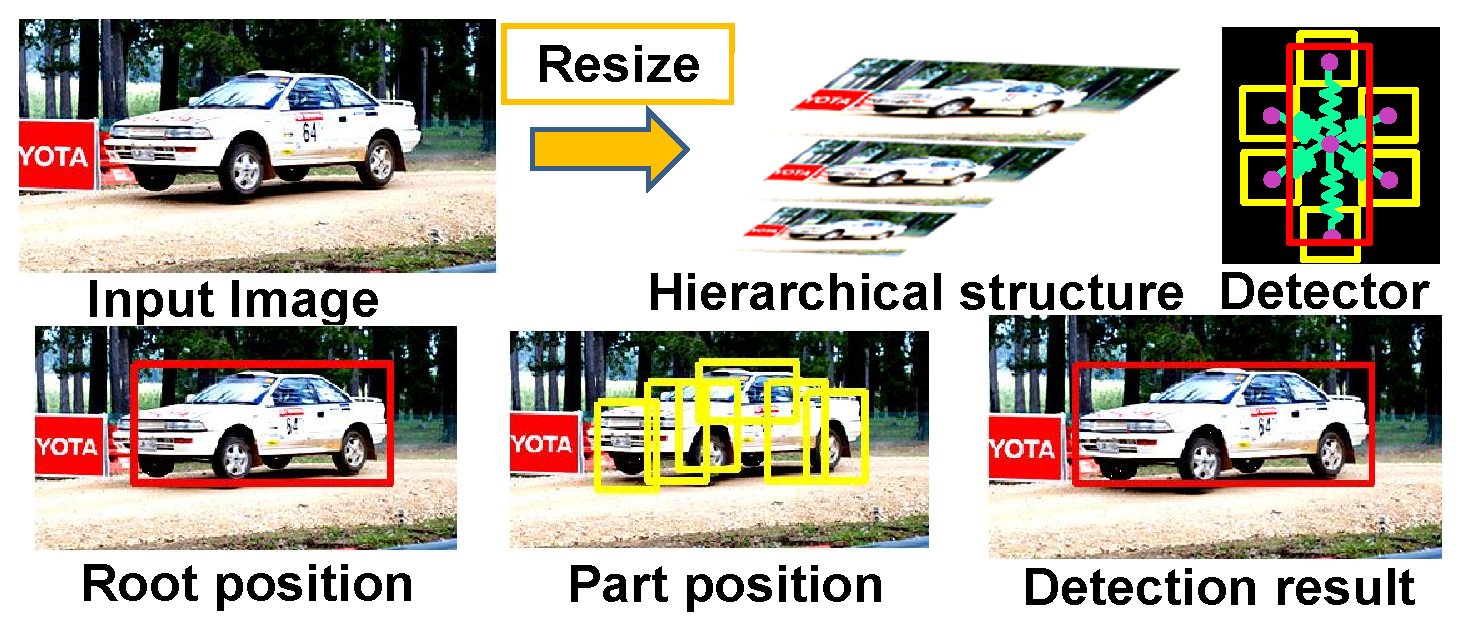
\includegraphics[width=0.95\hsize]{fig/deformable_model.eps}\\
  \caption{Vehicle detection flow with deformable models.}
  \label{fig:deformable_model}
 \end{center}
\end{figure}

Object detection often requires a machine learning phase to construct
the object models.
We assume that this learning phase has already been done a priori and
the object models are stored in the system.
Particularly we restrict our attention to vehicle detection in this
paper, utilizing the vehicle models provided by prior work
\cite{Niknejad12}.
A brief concept of this approach is illustrated in
Fig.~\ref{fig:deformable_model}.
Although these models achieve a high detection rate, the computational
cost of scoring similarity of an input image and the models using HOG
features is very expensive.
Specifically they include $2$ root filters and $12$ part filters, each
of which needs to be scored against $32$ resized images.
The scoring could be conducted for every squire of a few pixels
independently.
In consequence, there are approximately 10 million computational
blocks for a single high-definition image, while the frame-rate needs to
meet 10$\sim$20 frames per second (FPS) for practical use.
This data-parallel compute-intensive nature of HOG-based object
detection motivates the use of GPUs in this paper.

The CPU implementation of HOG-based vehicle detection has already been
developed in prior work \cite{Niknejad12}.
It leverages the POSIX \textit{pthread} to parallelize the scoring per
filter on a multicore CPU.
While we use this multicore implementation for a performance comparison
as it is, we also serialize it to execute on a single core so that we
can compare our GPU implementation to two variants of the CPU
implementation.
